\typeout{***********************************************************}
\typeout{* Dave Green's thesis template, based on the memoir class *}
\typeout{***********************************************************}
%==============================================================================%
% A PhD thesis template, based on LaTeX memoir class rather than the standard  %
% book class, as memoir offers many additional configuration options.          %
%                                                                              %
% For documentation on the memoir class, and other packages, see:              %
%                                                                              %
%   http://www.ctan.org/search/                                                %
%                                                                              %
% Dave Green --- MRAO --- 2016 September (Version 1.12)                        %
%==============================================================================%
% load the memoir class with basic options ...
%
\documentclass[a4paper,11pt,twoside,extrafontsizes,oldfontcommands]{memoir}
%
% load the thesis package, which sets various options for the memoir
% package, loads other packages (e.g. setting up fonts), and sets up
% various commands ...
%
% note: you will have to edit thesis.sty if you want to change things ...
%
\usepackage{thesis}
%
% other settings...
%
%\listfiles     % uncomment if needed for debugging ...
%------------------------------------------------------------------------------%
% For limited processing, list (with commas) selected files to process...
%
%\includeonly{CHAP-1/chapter1,APP-A/appendixa}
%
\begin{document}
%==============================================================================%
\frontmatter
%------------------------------------------------------------------------------%
\pagestyle{empty}
%
% titlepage ...
%
\ifpdf
  \pdfbookmark[0]{Titlepage}{title}{}
\fi
%
% note: include adjustment of baseline to ensure it looks
%       sensible if it is more than one line long,
%
\begin{center}
 \qquad\\[10mm]
 {\renewcommand\baselinestretch{1.2}\Huge\textbf{
%
% if more than one line, use "\\" to start a new line...
%
   Dave Green's thesis template
%
 }\par}
 \qquad\\[50mm]
 {\LARGE Andrew James Strange}\\[10mm]
 {\large School of Physics and Astronomy}\\[10mm]
 
\includegraphics[width=50mm]{UniOfManchesterLogo.png}\\[30mm]
 {\Large 2017 September}\\[10mm]
 {\large A thesis submitted to the University of Manchester \\ for the degree of Master of Science \\ in the Faculty of Engineering and Physical Sciences}
\end{center}

\cleardoublepage

\endinput

%
\pagestyle{plain}
%
% summary ...
%
\chapter*{Summary}

\addcontentsline{toc}{chapter}{Summary}

Here is my template for PhD or other theses, for pdf\LaTeX\ (or \LaTeX,
but pdf\LaTeX\ provides better internal hyperlinks).

It is based on the `\href{http://www.ctan.org/pkg/memoir}{memoir}'
\LaTeX\ class, which has a lot of useful features/options built-in. The
documentation for the memoir class says that `[it] provides the
functionality of over thirty of the more popular packages, thus
simplifying document sources'.

If there is any specific typesetting feature you want to use in your
thesis, you should first check in the comprehensive manual for the
memoir class via the link above (which has a detailed index). It may
well be that what you want is already provided by the memoir class (and
it is better to use its built-in capabilities, rather than loading
additional style files, unless you have to).

The rest of this template show various examples of features available.

See \url{http://www.mrao.cam.ac.uk/~dag/THESIS/} for the current version
of this template. (This version is V1.12, dated 2016 September).

\cleardoublepage

\endinput

%
% contents ...
%
%
% thesis.sty redefines \baselinestretch for larger line spacings, but
% here do not use this for the table of contents ...
%
\bgroup
\renewcommand{\baselinestretch}{1.0}\normalsize

\tableofcontents

%
% reset to default linespacing ...
%
\vspace{10mm}
\textit{Word Count: 16858}
\egroup

\cleardoublepage

\endinput

%
% declaration ...
%
\chapter*{Declaration}

\addcontentsline{toc}{chapter}{Declaration}

No portion of the work referred to in the dissertation has been submitted in support of an application for another degree or qualification of this or any other university or other institute of learning.

\cleardoublepage

\endinput

%
% thanks ...
%
\chapter*{Acknowledgements}

\addcontentsline{toc}{chapter}{Acknowledgements}

This dissertation has been produced with guidance and support from many people, without which it would not have seen the light of day.

Primarily, I must thank my supervisor Andy Pilkington. His guiding hand and experience over the course of this project has at times been the only thing keeping it on the straight and narrow. I am indebted to his help and his willingness to put up with me over the course of this year, and this work is built around the backbone he provided.

Secondly, thanks to the Manchester Particle Physics group, for providing a terrific environment for work, for all of the guidance and for all of the socialising. Particular mention must go to my colleagues on the ATLAS project; Jacob, Jonathan
, Yaadav and Agni for all of their invaluable experience and assistance throughout the year. Additionally, I must thank Sabah for providing me with his help and knowledge without hesitation when I needed it.

From my time at undergraduate, I must thank all my friends, who while provided encouragement and support from all the myriad of locations around the world they've run off to, and I must thank my undergraduate Director of Studies, Dave Green, for his advice during my time under his watch and for permitting me to use his \LaTeX template.

Finally however, none of this would have occurred were it not for the support of my dad, mum and brother. Their unwavering and tireless support, endless encouragement and motivating prods and willing to put up with whatever inconvenience I could give them carried this work through to its close.

To all those mentioned here, I owe you the most sincere gratitude. Thank you for everything.
\cleardoublepage

\endinput

%------------------------------------------------------------------------------%
\mainmatter
%------------------------------------------------------------------------------%
% Note: \graphicspaths is set to point to appropriate places to find
% figures for each Chapter or Appendix ...
%
\pagestyle{headings}
%
% chapters ...
%
\graphicspath{{CHAP-1/FIGS/}{.}}
\chapter{Basic use of the template}\label{c:first}

\section{Introduction}\label{s:firstfirst}

Starting from the (unpacked) template, you need to edit the
\verb|thesis.tex| file to point to: (i) all the `frontmatter' you want
(titlepage, summary, etc); (ii) your particular chapters and appendices;
(iii) the `backmatter' (i.e.\ references). Note that when drafting, if
you want to process one or a few chapters only, edit the
`\verb|\includeonly{...}|' line in \verb|thesis.tex| as needed. (Further
commands that may be useful when writing your draft thesis are discussed
in Chapter~\ref{c:drafting}.)

\section{Style options}

Many aspects of the style of the thesis are set in \verb|thesis.sty|,
which you can change as you want, and some of the possibilities are
explained in the comments in the file. These include:
%
\begin{enumerate}
%
\item chapter/section styles (see Chapter 6 of the
\href{http://www.ctan.org/pkg/memoir}{memoir} user manual, or the
\href{http://www.ctan.org/pkg/memoirchapterstyles}{memoirchapterstyles}
\LaTeX\ package for other styles) or specify a custom chapter style;
%
\item page header style (e.g.\ uppercase or not, underlined or not);
%
\item the default fonts use the `newtxtext' and `newtxmath' packages,
which provide a full range of Times based fonts for text and mathematics
-- see Section~\ref{s:mathsfonts} for examples -- or you can choose
other font packages;
%
\item the colours used for different types of hyperlinks (which are
defined in \verb|thesis.sty| using the \verb|\hypersetup{...}| command;
you can change to use darker colours or dark grey -- e.g.\ for
printing -- be uncommenting the appropriate lines in \verb|thesis.sty|).
%
\end{enumerate}
%
There are various other settings in \verb|thesis.sty|, which you can
also adjust if you want, but I expect you are likely to stick with the
defaults (e.g.\ the vertical spacing and label style of lists; the page
size; the default figure/table captions font size/width; whether to list
the bibliography in table of contents; what level of
sections/subsections to list -- numbered or not -- in the table of
contents; use lowercase letters for footnote labels; line spacing;
vertical page formatting; settings controlling the display of
figures/tables on a page).

\section{References}

The `natbib' package\footnote{e.g.\ see
\url{http://merkel.zoneo.net/Latex/natbib.php} for a reference list of
the commands.} is loaded by \verb|thesis.sty| and various settings
`natbib' are made -- which are conventional for astronomical references.
Here are some example references, \citet{1971QJRAS..12...10S,
2002ISAA....5.....S, 2003JAHH....6...46S}, and here are some more in
parentheses \citep{2005JHA....36..217S, 2009JHA....40...31S}.

\section{URLs}

This illustrates how to give a url \url{http://www.google.com/}, using
the \verb|\url{...}| command. (Or you can provide a link using some
\href{http://www.google.com/}{text}, which does not show the URL --
which is probably not a good idea for a thesis -- using the
\verb|\href{...}{...}| command.)

\section{Mathematical fonts}\label{s:mathsfonts}

The following illustrate some equations and the mathematical fonts
available.
%
\begin{enumerate}
%
\item Mathematical symbols, as sloping font, including greek letters:
$$
  a^2 + b^2 = c^2, \qquad
  A^2 + B^2 = C^2, \qquad
  \alpha + \beta = \gamma, \qquad
  \Gamma + \Delta = \Omega.
$$
\item Vectors, as a bold sloping font (using \verb|$\vec{...}$|):
$$
  a = \vec{b} \cdot \vec{c}, \qquad
  A = \vec{B} \cdot \vec{C}, \qquad
  \vec{\alpha} + \vec{\beta} = \vec{\gamma}, \qquad
  \vec{\Gamma} + \vec{\Delta} = \vec{\Omega}.
$$
(Note: the default letter \verb|$v$| looks
very similar to the greek \verb|$\nu$| -- $v$ compared with $\nu$ -- so
instead you can use \verb|$\varv$|, which looks like $\varv$.)
%
\item An integral:
$$
 a^2 + b^2 = \int_0^\infty x^2 \, \text{d}x.
$$
\item Upright greek letters are available. For example, with the `newtx'
fonts, use \verb|\upmu| (inside maths mode), for units (such as
$\upmu$m, or $\upmu$Jy~beam$^{-1}$); use \verb|\updelta| or
\verb|\upDelta| for increments (such as $\updelta x$, $\upDelta y$).
Also available is \verb|\uppartial| for an upright partial derivative,
such as $\uppartial y/\uppartial x$.
%
\end{enumerate}

\section{Astronomical abbreviations}

\subsection{Coordinates}

This illustrates several astronomical abbreviations that are defined in
\verb|thesis.sty| (as per journals), for use in maths mode only:
%
\begin{itemize}
%
\item \verb|$12\degr 34\arcmin 56\arcsec$| gives $12\degr 34\arcmin
56\arcsec$;
%
\item \verb|$12\fdg3, 45\farcm7, 78\farcs9$| gives $12\fdg3, 45\farcm7,
78\farcs9$;
%
\item \verb|$12\fh3, 45\fm7, 78\fs9$| gives $12\fh3, 45\fm7, 78\fs9$;
%
\item \verb|$12\fp3$| gives $12\fp3$.
%
\end{itemize}

\subsection{Ions}

Also defined is \verb|\ion{...}{...}| which can be used to specify
ionised states of atoms. For example, \verb|\ion{H}{II}| (or
\verb|\ion{H}{ii}|) gives `\ion{H}{II}'.

\newcommand\HII{\ion{H}{II}}

If you frequently use particular ions, you may want to define macros for
them in the preamble of your thesis (i.e.\ before the
\verb|\begin{document}| command). For example, including
\verb|\newcommand\HII{\ion{H}{II}}| defines the \verb|\HII| command,
which produces `\HII'. (Note: if you use `\verb|... \HII ...|' in a
sentence -- i.e.\ with a space after the \verb|\HII| -- then the space
will be swallowed by \LaTeX; instead use `\verb|... {\HII} ...|' to
preserve the following space.)

\section{Section/list formatting}

The rest of this chapter illustrates the formatting for sections,
sub-sections, sub-sub-sections, and lists (both enumerated or not).

\subsection{A subsection}

Here is some sample text. Here is some sample text. Here is some sample
text. Here is some sample text. Here is some sample text. Here is some
sample text. Here is some sample text. Here is some sample text. Here is
some sample text. Here is some sample text. Here is some sample text.
Here is some sample text.

\subsubsection{Here is a sub-subsection}

Here is some sample text. Here is some sample text. Here is some sample
text. Here is some sample text. Here is some sample text. Here is some
sample text. Here is some sample text. Here is some sample text. Here is
some sample text. Here is some sample text. Here is some sample text.
Here is some sample text.

\subsubsection{Here is another sub-subsection}

Here is some sample text. Here is some sample text. Here is some sample
text. Here is some sample text. Here is some sample text. Here is some
sample text. Here is some sample text. Here is some sample text. Here is
some sample text. Here is some sample text. Here is some sample text.
Here is some sample text. Here is some sample text. Here is some sample
text. Here is some sample text.

\subsection{Another subsection -- lists}

Here is some sample text. Here is some sample text. Here is some sample
text. Here is some sample text. Here is some sample text. Here is some
sample text. Here is some sample text. Here is some sample text. Here is
some sample text. Here is some sample text. Here is some sample text.
Here is some sample text.
%
\begin{enumerate}
%
\item Here is an example enumerated list. Here is an example enumerated
list. Here is an example enumerated list. Here is an example enumerated
list. Here is an example enumerated list. Here is an example enumerated
list.
%
\begin{enumerate}
%
\item Here is a second level list.
%
\item Here is an example enumerated list. Here is an example enumerated
list. Here is an example enumerated list.
%
\end{enumerate}
%
\item Here is an example enumerated list. Here is an example enumerated
list.
%
\item Here is an example enumerated list. Here is an example enumerated
list. Here is an example enumerated list. Here is an example enumerated
list.
%
\end{enumerate}
%
Here is some sample text. Here is some sample text. Here is some sample
text. Here is some sample text. Here is some sample text. Here is some
sample text.
%
\begin{itemize}
%
\item Here is an example  list. Here is an example list. Here is an
example  list. Here is an example list. Here is an example  list. Here
is an example list.
%
\item Here is an example  list. Here is an example list.
%
\item Here is an example  list. Here is an example list. Here is an
example  list. Here is an example list.
%
\end{itemize}
%
Here is some sample text. Here is some sample text. Here is some sample
text. Here is some sample text. Here is some sample text. Here is some
sample text.

\endinput

%
\graphicspath{{CHAP-2/FIGS/}{.}}
\chapter[Example tables and figures]{Second Chapter -- example tables
and figures -- which has a long title (too long for the
headline/contents)}\label{c:tables+figures}

\epigraph{`To err is human, but to really foul things up you
need a computer'}{\textit{anonymous}}

\section{Introduction}

This Chapter illustrates the addition of a quotation on the first page
of a Chapter (using the command \verb|\epigraph{...}{...}|). Also, this
Chapter has a long title -- which is too long for the page
headline/contents -- but a shorter alternative was specified for the
page headline/contents entry (using
%
\verb|\chapter[short title]{full title}|). Similarly shorter versions of
Section headings etc.\ can be specified, if needed..

The rest of this chapter illustrates various styles for tables and
figures.

\newcolumntype{d}[1]{D{.}{.}{#1}}
\newcommand{\dhead}[1]{\multicolumn{1}{c}{#1}}
%
\begin{table}
  \caption{This is a simple example table.}\label{t:simple}
  \medskip
  \centering
    \begin{tabular}{cd{1.3}d{2.0}}\hline
      number & \dhead{reciprocal} & \dhead{cube} \\\hline
        1    &     1      &    1   \\
        2    &     0.5    &    8   \\
        3    &     0.333  &   27   \\
        4    &     0.25   &   64   \\\hline
    \end{tabular}\\[5pt]
    Note: here is a note to the table.
\end{table}

\begin{table}
  \caption{This is a better example table.}\label{t:rules}
  \medskip
  \centering
    \begin{tabular}{cd{1.3}d{2.0}}\toprule
      number & \dhead{reciprocal} & \dhead{cube} \\\midrule
        1    &     1      &    1   \\
        2    &     0.5    &    8   \\
        3    &     0.333  &   27   \\
        4    &     0.25   &   64   \\\bottomrule
    \end{tabular}\\[5pt]
    Note: here is a note to the table.
\end{table}

\enlargethispage{\baselineskip} % to avoid `orphan' line

\section{Example tables}

Table~\ref{t:simple} and Table~\ref{t:rules} are example tables that
illustrate the use of the `\verb|d|' column specifier -- which is
defined in the \verb|.tex| source -- to align numbers by decimal places
(as the `memoir' class emulates the `dcolumn' package).

The difference between them is that Table~\ref{t:simple} uses the
default horizontal rules (i.e.\ \verb|\hline|), whereas
Table~\ref{t:rules} uses alternate rules with better vertical spacing
(i.e.\ \verb|\toprule|, \verb|\midrule| and \verb|\bottomrule|), from
the `booktabs' package, which are emulated by the memoir class.

If you have a long table that spans more that one page, then use the
\href{http://www.ctan.org/pkg/longtable}{longtable} package. You will
need to process the table through (pdf)\LaTeX\ several times for the
`longtable' algorithm that decides on the column widths to converge.
Landscape multiple-page tables can also be produced using `longtable',
provided you also load the `pdflscape' package and place the table
within \verb|\begin{landscape}| and \verb|\end{landscape}|. In both
cases you will probably want to specifiy the caption width. Specify
either \verb|\setlength{\LTcapwidth}{\linewidth}| or
\verb|\narrowcaptionwidth| and
\verb|\setlength{\LTcapwidth}{\thesiscaptionwidth}|. If using the
\verb|landscape| environment, place these commands just after
\verb|\begin{landscape}|.

\section{Example figures}

This section illustrates various figure styles. Figure~\ref{f:fullwidth}
shows a figure with a full width caption (using
\verb|\normalcaptionwidth|), whereas Figure~\ref{f:narrow} shows the
slightly narrower caption width (\verb|\narrowcaptionwidth|, which is
the default). Figure~\ref{f:labels} shows how to add `a)', `b)' $\dots$
labels to a figure with contains several sub-figures.
Figure~\ref{f:landscape} shows a landscape figure (also using
\verb|\normalcaptionwidth|). Finally Figure~\ref{f:2x2} shows an
$2\times2$ array of sub-figures, with the caption in one corner (which
needs \verb|\normalcaptionwidth|).

\begin{figure}
%
\centerline{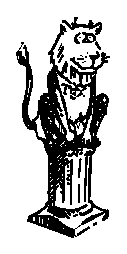
\includegraphics[width=3cm]{testfig}}
%
\medskip
%
\normalcaptionwidth\caption{This shows a figure with a full width
caption. Here is some sample text. Here is some sample text. Here is
some sample text. Here is some sample text. Here is some sample text.
Here is some sample text. Here is some sample text. Here is some sample
text. Here is some sample text.\label{f:fullwidth}}
%
\end{figure}

\begin{figure}
%
\centerline{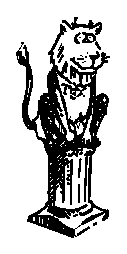
\includegraphics[width=3cm]{testfig}}
%
\medskip
%
\caption{This shows a figure with a narrow width caption. Here is
some sample text. Here is some sample text. Here is some sample text.
Here is some sample text. Here is some sample text. Here is some
sample text.\label{f:narrow}}
%
\end{figure}

\begin{figure}
%
\centerline{\hbox to 8cm{\large a)\hfill}}
\centerline{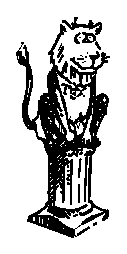
\includegraphics[angle=90,width=8cm]{testfig}}
\medskip
\centerline{\hbox to 8cm{\large b)\hfill}}
\centerline{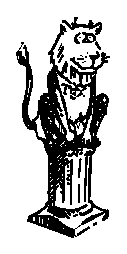
\includegraphics[angle=-90,width=8cm]{testfig}}
\medskip
%
\caption{This shows a figure with including `a)' and `b)' labels
for the sub-figures. Here is some sample text. Here is some sample text.
Here is some sample text. Here is some sample text. Here is some
sample text. Here is some sample text.\label{f:labels}}
%
\end{figure}

\begin{sidewaysfigure}
%
\centerline{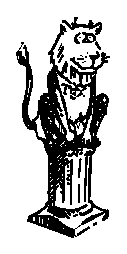
\includegraphics[width=5cm]{testfig}}
\medskip
%
\normalcaptionwidth\caption{This shows a sideways figure (with
full width caption). Here is some sample text. Here is some sample
text. Here is some sample text. Here is some sample text. Here is
some sample text. Here is some sample text.\label{f:landscape}}
%
\end{sidewaysfigure}

\begin{figure}
%
\begin{tabular}{p{6cm}cp{6cm}}
%
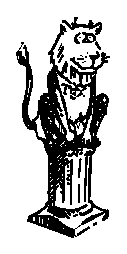
\includegraphics[width=2cm,angle=45]{testfig} & &
  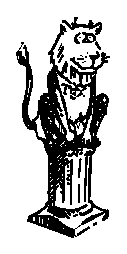
\includegraphics[width=2cm,angle=315,origin=c]{testfig} \\[15pt]
%
\raisebox{-\height}{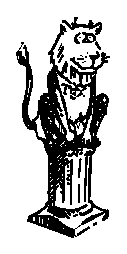
\includegraphics[width=2cm,angle=315,origin=c]{testfig}}
  & &
%
\normalcaptionwidth\caption{This shows an array of sub-figures
(with a caption in the array). Here is some sample text. Here is some
sample text. Here is some sample text. Here is some sample text. Here is
some sample text. Here is some sample text.\label{f:2x2}}
%
\end{tabular}
%
\end{figure}

\endinput

%
\graphicspath{{CHAP-3/FIGS/}{.}}
\chapter{Useful commands for drafting}\label{c:drafting}

\section{Introduction}

This Chapter discusses various commands -- some built into the memoir
class, others defined in \verb|thesis.sty|, and some requiring
additional packages to be loaded -- which may be useful when drafting.
These include:
%
\begin{enumerate}
%
\item marginal notes (see Section~\ref{s:notes});
%
\item marginal marks to indicate changes/deletions/additions (see
Section~\ref{s:changes});
%
\item the addition of line numbers (see Section~\ref{s:lineno});
%
\item adding a `watermark' on each page, to timestamp a particular
version (see Section~\ref{s:watermark}).
%
\end{enumerate}

\section{Marginal notes}\label{s:notes}

The \verb|thesis.sty| file defines the \verb|\note{...}| command for
marginal notes\note{this is an example marginal note} (in a small font,
black). In addition \verb|\todo{...}| and \verb|\tocheck{...}| are
defined for specific notes/reminders on items still to do or check,
which are shown as marginal notes in red and blue respectively, which
are illustrated below.

Here is some sample text.
%
\todo{here is a note of something still to do}
%
Here is some sample text. Here is some sample text. Here is some sample
text. Here is some sample text. Here is some sample text. Here is some
sample text. Here is some sample text. Here is some sample text. Here is
some sample text.
%
\tocheck{here is a note about something to check}
%
Here is some sample text. Here is some sample text. Here is some sample
text. Here is some sample text. Here is some sample text. Here is some
sample text. Here is some sample text. Here is some sample text. Here is
some sample text. Here is some sample text.

\section{Changes/deletions/additions}\label{s:changes}

The memoir class provides commands to mark changes, deletions or
additions made, i.e.\ \verb|\changed{...}|, \verb|\deleted{...}| and
\verb|\added{...}| (see Chapter~18 of the 
\href{http://www.ctan.org/pkg/memoir}{memoir} user manual for
details). These add symbols with a text label to the margin to indicate
revisions have been made (that is provided \verb|\changemarks| rather
than \verb|\nochangemarks| is used, and that the \verb|draft| option is
used, or \verb|\draftdoctrue| is set -- otherwise these change marks are
not shown).

Here is some sample text.\deleted{label} Here is some sample text. Here
is some sample text. Here is some sample text. Here is some sample text.
Here is some sample text. Here is some sample text.
Here is some sample text.\added{text} Here is some sample text.
Here is some sample text. Here is some sample
text. Here is some sample text. Here is some sample text. Here is some
sample text.\changed{label text} Here is some sample text. Here is some
sample text.

In addition, \verb|thesis.sty| defines a command \verb|\fixed{...}|
which can be used to mark changed text, in green (along with `***' 
added in the
margin).

Here is some sample text. Here is some sample
text. \fixed{Here is some `fixed' text. Here is some `fixed' text. Here
is some `fixed' text.} Here is some sample text.

\section{Additional packages for drafting}

\subsection{Add line numbers}\label{s:lineno}

If you want to number the lines when drafting, then you can use the
`lineno' package. This is included towards the end of \verb|thesis.sty|,
but is commented out. If you want to use this package, the uncomment it
in \verb|thesis.sty|. Then you can switch linenumbers on or off with
\verb|\linenumbers| or \verb|\nolinenumbers|. You can reset the line
numbers -- for example if you want to number the lines in each chapter
from one -- using \verb|\resetlinenumbers|.

\subsection{Add a `watermark'}\label{s:watermark}

If you want to add a `watermark' to each page, to indicate the time/date
of the draft version, you can use the `draftwatermark' package. This is
included towards the end of \verb|thesis.sty| -- along with commands to
setup a faint grey `watermark' in the left margin of each page saying
`draft' with the date and time -- but is commented out. Uncomment and
edit as needed the relevant lines in \verb|thesis.sty| if you want to
use a watermark when drafting.

\endinput



%
% appendices...
%
\appendix
%
\graphicspath{{APP-A/FIGS/}{.}}
\addtocontents{toc}{\clearpage}

\chapter{This is an appendix}

\section{Introdution}

This is an example Appendix, with a couple of Sections. (The
\verb|.tex| for this Appendix starts with
\verb|\addtocontents{toc}{\clearpage}| to force a new page in the Table
of Contents. You may want to use this -- at the final stage -- if the
page breaks in your Table of Contents are in awkward places.)

\section{Another section}

Here is some sample text. Here is some sample text. Here is some sample text.
Here is some sample text. Here is some sample text. Here is some sample text.
Here is some sample text. Here is some sample text. Here is some sample text.
Here is some sample text. Here is some sample text. Here is some sample text.

\endinput

%
\graphicspath{{APP-B/FIGS/}{.}}
%
% Given this uses \includepdf, only process if using pdflatex ...
%
\ifpdf

\chapter{Another appendix -- a Paper}

This Appendix shows how to include another .pdf document (e.g.\ in this
case, the first three pages a paper), using the \verb|\includepdf{...}|
command from the \href{http://www.ctan.org/pkg/pdfpages}{pdfpages}
package. This requires processing with pdf\LaTeX\
rather than \LaTeX.

%
% include .pdf version of a paper...
%
% \includepdf (the pdfpages package) is used to include the .pdf
%   (note, "pages=-" means all pages, or specific pages can be included)
%   scaled and framed, and with a speficied pagestyle command...
% \markboth is used to specify top labels on odd/even pages
%

\clearpage

\makepagestyle{papers}
\makeevenhead{papers}{}{}{\rightmark}
\makeoddhead{papers}{\leftmark}{}{}
\makeevenfoot{papers}{}{\thepage}{}
\makeoddfoot{papers}{}{\thepage}{}

\markboth{My `cubehelix' paper}{My `cubehelix' paper}

\includepdf[pages=1-3,scale=0.82,frame=true,
   pagecommand=\thispagestyle{papers}]{cubehelix-paper.pdf}

%
% else...
%
\else

\chapter{Another appendix}

As this was processed with \LaTeX, not pdf\LaTeX, this does
not show the inclusion of a \verb|.pdf| document.

%
% end of \ifpdf ...
%
\fi

\endinput

%------------------------------------------------------------------------------%
\backmatter
%------------------------------------------------------------------------------%
% references...
%
% 1) For an easy way to construct \bibitem entries for use by natbib, see
% Section 5 of basisample available from:
%
%    http://astron-soc.in/bulletin/instructions.php
%
% If ADS *is* use to construct \bibitem text from a private library, then
% also load the fixads.sty package (from DAG), which will
%  a) remove the `Oxford comma' in three author papers;
%  b) for an bibcode containing an "&", will set up an alias using
%     a "+" instead, which can be used in the tabular environment.
%
% 2) LaTeX will give a warning if you cite a paper for which there is no
%    \bibitem entry, but not the other way around. To check to see if
%    you have \bibitem entry that is not cited, use the check-cites.sty
%    package (from DAG).
%
%------------------------------------------------------------------------------%
%\setlength{\bibsep}{0pt}            % vertical spacing between references
%\renewcommand{\bibname}{References} % instead of "Bibliography"

%
%                *****************
% Alternatively, if you use BibTeX, either:
%                *****************
%
% 1) put the appropriate .bib file in the sub-directory below the main
% thesis directory, where this file is (e.g. "OTHER/"), then uncomment
% the following two lines, and edit as needed for the required
% \bibliographystyle and \bibliography:
%
\bibliographystyle{OTHER/atlasBibStyleWithTitle}        % <- add required style
\bibliography {OTHER/ref}       % <- add name of .bib file
%
% or
%
% 2) put the appropriate .bib file in directory, where the main .tex
% file is, and put the \bibliographystyle{...} and \bibliography{...}
% at the end of the main .tex file.
%

\endinput

%
% or, if you are using BibTeX, and you .bib file is in your main thesis
% directory, then edit/uncomment these lines
%
%\bibliographystyle{...}    % your .bst bibliography style
%\bibliography{...}         % your bibliography
%==============================================================================%
\end{document}
